%tag:0007
%label:"art:heegaardDiagrams"
%author:JeffHicks
%name:"Heegaard Diagrams:combinatorial descriptions of 3 manifolds"
%type:"article"


%label:"def:heegaardSplitting"
%author:JeffHicks
%name:"Heegaard splitting"
%type:"definition"
%indepth:art:heegaardDiagram
%example:exm:heegaardSplitting


    Let $M$ be a closed 3-manifold. A \emph{genus $g$} Heegaard splitting of $M$ is a decomposition
    \[M=U_1\cup_{\Sigma_g} U_2\]
    where $U_1, U_2$ are genus $g$ handlebodies along with an identification of their boundaries (the surface $\Sigma_g)$ with a diffeomorphism.

%parent:"def:heegaardSplitting"
%author:JeffHicks
%name:"Heegaard splitting"
%type:"example"
%indepth:art:heegaardDiagram
%label:"exm:heegaardSplitting"


    Consider the 3-sphere
    \[M=S^3=\left\{(x_0, x_1, x_2, x_3)\st x_i\in \RR, \sum_{i=1}^3 x_i^2=1.\right\}\]
    Consider the decomposition of this into two halves along the $z_0$ coordinate:
    \begin{align*}
        U_1=\{(x_0, x_1, x_2, x_3)\in S^3 \st x_0\leq 0\}&& U_2=\{(x_0, x_1, x_2, x_3)\in S^3 \st x_0\geq 0\}
    \end{align*}
    Then both $U_1, U_2$ are diffeomorphic to the 3-ball, and are glued together by their common boundary $S^2=\Sigma_0$. See \cref{fig:heegaardSplitting}.
    %parent:def:heegaardSplitting
%author:JeffHicks
%name:"Heegaard splitting for $S^3$"
%type:"figure"
%indepth:art:heegaardDiagram
%label:"fig:heegaardSplitting"
%parent:"exm:heegaardSplitting"
%caption:"After identifying $S^3\setminus \{(1, 0, 0, 0)\}$ with $\RR^3$ via stereographic projection, the Heegaard splitting of $S^3$ is given by taking the unit sphere, which decomposes the sphere into two $3$-balls. We also draw the meridinal line $(\cos(\theta), \sin(\theta), 0, 0)$."



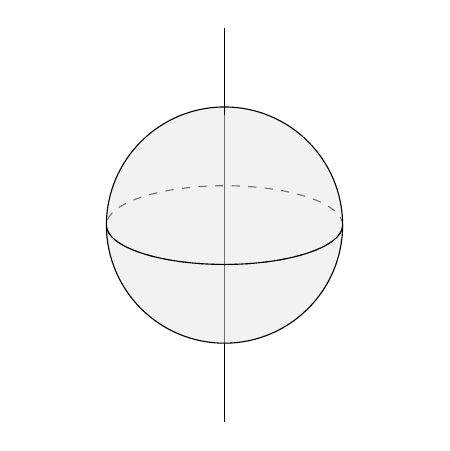
\begin{tikzpicture}
    \draw (-0.5,2) -- (-0.5,-3);
    \draw[dashed]  (-0.5,-0.5) ellipse (1.5 and 0.5);
    \draw[fill=gray!20, fill opacity=.5]  (-0.5,-0.5) ellipse (1.5 and 1.5);
    
    \draw (-0.5,2) -- (-0.5,0.9);
    
    \clip  (2,-0.5) rectangle (-3,-1.5);
    \draw  (-0.5,-0.5) ellipse (1.5 and 0.5);
    \end{tikzpicture}
    \label{exm:heegaardSplitting}

A handlebody is a 3-manifold $U$ with boundary with a collection disks $\{f_i: D^2\to U\}_{i=1}^g$ which are embedded and disjoint, so that $U\setminus \bigcup_{i=1}^g \Im(f_i)=D^3$. 
%tag:000T
%label:"lem:handlebodies"
%author:JeffHicks
%name:"Morse functions for handlebodies"
%type:"lemma"


    Let $U$ be a 3-manifold with boundary. $U$ is a handlebody if and only if there exists a Morse function $f: U\to \RR$ whose 
    \begin{itemize}
        \item Gradient $\nabla f$ points outward along the boundary of $U$;
        \item $f$ has only critical points of index $0$ and $1$.
    \end{itemize}
    \label{lem:handlebodies}

%label:"prp:existenceOfHeegaardSplitting"
%author:JeffHicks
%name:"existence of Heegaard splitting"
%type:"proposition"



    Let $M$ be a closed 3-manifold. There exists a Heegaard splitting for $M$.
    \label{prp:existenceOfHeegaardSplitting}

%label:"proof:existenceOfHeegaardSplitting"
%author:JeffHicks
%name:"existence of Heegaard splitting"
%type:"proof"
%parent:prp:existenceOfHeegaardSplitting


    Let $f: M\to \RR$ be a self indexing Morse function. Consider the level set $f^{-1}(1.5)$. Because $1.5$ is not a critical value of $f$, this is a smooth surface $\Sigma_g\subset M$. Let $U_1=f^{-1}([0, 1.5])$ and let $U_2=f^{-1}([1.5, 3])$. By \cref{lem:handlebodies}, these are handlebodies.

To determine the data of a Heegaard splitting, one must specify the data of two fillings of $\Sigma_g$ by handlebodies. When the Heegaard splitting is determined by a self-indexing Morse function $f: M\to \RR$, we can use the critical points to determine the fillings $U_1$ and $U_2$ based on data contained in $\Sigma_g$. The filling $U_1$ is constructed by considering how the downward flow spaces of the critical points of $f|_{U_1}$ attach to the $\Sigma_g$. We may additionally assume  that $f$ has a unique maximum; then to determine the filling we only need to consider how $W^\downarrow(p)$ intersects $\Sigma_g$ for $\{p\in \Crit(f), \ind(p)=1\}$. Furthermore, there are $g$ such critical points which we enumerate as $\{p_i\}_{i=1}^g$. These downward flow spaces are 2-dimensional, so $\{\Sigma_g\cap W^\downarrow(p_i)\}_{i=1}^g$ gives $g$ disjoint cycles in $\Sigma_g$. We call these cycles 
\[\{\alpha_i\}_{i=1}^g:=\{ W^\downarrow(p_i)\cap \Sigma_g\}_{p_i\in \Crit(f), \ind(p_i)=1}\]
Similarly, we can consider the index 2 critical points of $f$, which are all contained in $U_2$, and look at their upward flow spaces
\[\{\beta\}_{i=1}^g:=\{ W^\uparrow(p_i)\cap \Sigma_g\}_{p_i\in \Crit(f), \ind(p_i)=1}.\]
%tag:0007
%label:def:heegaardDiagram
%author:JeffHicks
%name:"Heegaard diagram"
%type:definition


    A \emph{Heegaard diagram} is a triple $(\Sigma_g, \{\alpha_i\}_{i=1}^g, \{\beta_i\}_{i=1}^g$). Here, $\Sigma_g$ is a genus $g$ surface and $\{\alpha_i\}_{i=1}^g, \{\beta_i\}_{i=1}^g$ are collections of smooth 1-cycles in $\Sigma_g$ such that
    \begin{itemize}
         \item $\Sigma_g\setminus \{\alpha_i\}_{i=1}^g, \Sigma_g\setminus \{\beta_i\}_{i=1}^g$ are connected and;
         \item $\alpha_i\cap \alpha_j=\emptyset = \beta_i \cap \beta_j$ whenever $i\neq j$.
    \end{itemize}

We will usually write $\underline \alpha, \underline \beta$ for $\{\alpha_i\}_{i=1}^g, \{\beta_i\}_{i=1}^g$.
%label:exm:heegaardDiagram3Sphere
%author:JeffHicks
%name:"Heegaard diagram for $S^3$"
%type:example
%todo:"add a picture"


    \label{exm:heegaardDiagram3sphere}
    Consider the 3-sphere 
    \[S^3=\{(z_1, z_2)\;|\; z_i\in \CC, |z_1|^2+|z_2|^2=1\}\]. We first describe a Heegaard diagram for $S^3$. Take the function $f=|z_1|^2-|z_2|^2$, and consider the sets 
    \begin{align*}
        U_1=f^{-1}([0, 1]) && U_2=f^{-1}([-1, 0])
    \end{align*}
    These sets are fillings of the boundary 
    \[\Sigma_1:=f^{-1}(0)=\left\{(z_1, z_2)\;|\; |z_1|^2=\frac{1}{2}, |z_2|^2=\frac{1}{2}\right\}=\{(e^{i\theta_1}, e^{i\theta_2}), \theta_1, \theta_2\in S^1\}.\]
    which is a torus. Observe that $\grad f$ is transverse to the boundary of $\Sigma_1$, and that the critical locus of $f$ can be parameterized by the cycles $\{(e^{i\theta_1}, 0)\}\sqcup \{(0, e^{i\theta_2})\}$. It follows the sets $U_1, U_2$ are diffeomorphic to $S^1\times D^2$ and $D^2\times S^1$ respectively. These are handlebodies, giving us a Heegaard decomposition.

    We now Morsify $f$ by taking a perturbation. Take $\rho:[-1, 1]\to [0, \eps]$ satisfying the constraints:
    \begin{align*}
        \rho|_{[-1, -.5]}=\eps/10 && \rho|_{[0, 1]}=0 && |\rho'|<\eps
    \end{align*}
    The the function $f+ \rho(f)\cos(\theta_1)+\rho(-f)\cos(\theta_2)$ has 4 critical points at $(\pm 1 , 0)$ and $(0, \pm 1)$. The attaching disks associated to the index 2 and index 1 critical points give the  cycle $\alpha_1=S^1\ times \{1\}$ and $\beta_1=\{1\}\times S^1$ inside $T^2$. 

Every Heegaard diagram specifies a 3-manifold, however a single 3-manifold can have many different presentations with different Heegaard diagrams. We have already seen 2 different Heegaard diagrams for $S^3$ in \cref{exm:heegaardSplitting} and  \cref{exm:heegaardDiagram3sphere}. 
Therefore, if we are to study 3-manifolds via their Heegaard diagram, we need to understand when two diagrams give presentations of the same manifold. We first describe some operations which modify a Heegaard diagram, but produce the same 3-manifold. 
%label:def:heegaardStabilization
%author:JeffHicks
%name:"Heegaard stabilization"
%type:definition


    Let $(\Sigma_g, \{\alpha_i\}_{i=1}^g, \{\beta_i\}_{i=1}^g)$ be a Heegaard diagram. Let $p\in \Sigma_g$ be a point avoiding the cycles $\alpha_i, \beta_i$. The \emph{stabilization of $\Sigma_g$ at $p$} is the diagram $(\Sigma_g \#_p T^2, \{\alpha_i\}_{i=1}^{g+1}, \{\beta_i\}_{i=1}^{g+1})$ where $\alpha_{g+1}, \beta_{g+1}$ are the meridional and longitudinal classes of $T^2$.

%label:"rem:heegaardStabilizations"
%author:JeffHicks
%name:"Morse interpretation of Heegaard stabilization"
%type:"remark"
%parent:"def:heegaardStabilization"

One way to see that stabilization of a Heegaard diagram produces the same manifold comes from Morse theory. Consider $\Sigma_g$ as the level set of a self-indexing Morse function $f$. Suppose that we wanted to modify our Morse function to $\tilde f$ by adding in a pair of critical points $p, q$ so that $\ind(p)=1$ and $\ind(q)=2$. We imagine that the critical points would appear on opposite sides of $\Sigma_g$, and be connected by a single flow line. Furthermore, $\tilde \Sigma_{g+1}=\tilde f(1.5)$, the new level set, would be of genus $g+1$. By applying surgery along either the attaching circles $W^\downarrow(p)\cap \tilde \Sigma_{g+1}$ or $W^\uparrow(q)\cap \tilde \Sigma_{g+1}$, we obtain $\Sigma_g$. See \cref{fig:heegaardStabilization}.
%label:"fig:heegaardStabilization"
%author:JeffHicks
%name:"rounding corner in Polterovich surgery"
%type:"figure"
%parent:"thm_roundingCorner"
%caption:"From the perspective of Morse theory, stabilization comes from the creation of a pair of cancelling critical points."



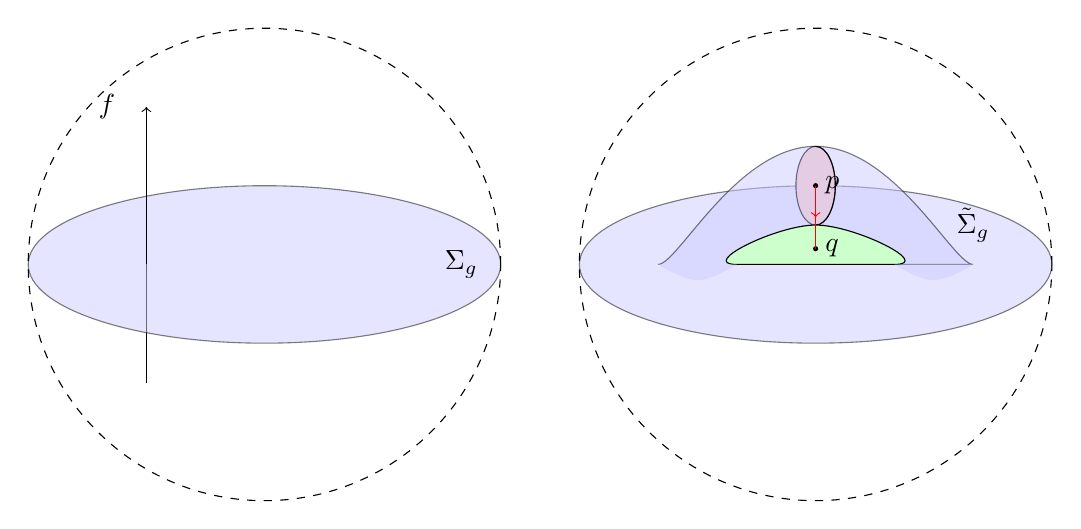
\begin{tikzpicture}
    \draw (-4,-1) -- (-4,0.5) ;
    \draw[opacity=.5,fill= blue!20]  (-2.5,0.5) ellipse (3 and 1);
    \draw[opacity=.5, fill=blue!20]   (4.5,0.5) node (v1) {} ellipse (3 and 1);
    \draw (6,-2);
    \draw[->](-4,0.5) -- (-4,2.5);
    \node at (-4.5,2.5) {$f$};
    \node at (0,0.5) {$\Sigma_g$};
    \draw[dashed]  (-2.5,0.5) ellipse (3 and 3);
    \draw[dashed]  (v1) ellipse (3 and 3);
    \draw[fill=red!20]  (4.5,1.5) ellipse (0.25 and 0.5);
    \draw[opacity=.5, fill=blue!20] (2.5,0.5) .. controls (2.75,0.5) and (3.5,2) .. (4.5,2) .. controls (5.5,2) and (6.25,0.5) .. (6.5,0.5) .. controls (6.25,0.5) and (6.25,0.5) .. (5.5,0.5) .. controls (5.75,0.5) and (5,1) .. (4.5,1) .. controls (4,1) and (3.25,0.5) .. (3.5,0.5);
    
    \node[right] at (4.5,1.5) {$p$};
    \node[fill=black, circle, scale=.2] at (4.5,1.5) {};
    \begin{scope}[]
    
    \clip  (5,1) rectangle (4.5,2);
    \draw  (4.5,1.5) ellipse (0.25 and 0.5);
    \end{scope}
    
    
    
    \draw[fill=green!20] (3.5,0.5) .. controls (3,0.5) and (4,1) .. (4.5,1) .. controls (5,1) and (6,0.5) .. (5.5,0.5)--cycle;
    \node[right] at (4.5,0.7) {$q$};
    \node[circle, fill=black, scale=.2] at (4.5,0.7) {};
    
    \begin{scope}[]
    
    \fill[opacity=.5, fill=blue!20]  plot[smooth, tension=.7] coordinates {(2.5,0.5) (3,0.3) (3.5,0.5)};
    
    \end{scope}\begin{scope}[shift={(3,0)}]
    
    \fill[opacity=0.5, fill=blue!20]  plot[smooth, tension=0.7] coordinates {(2.5,0.5) (3,0.3) (3.5,0.5)};
    
    \end{scope}\node at (6.5,1) {$\tilde \Sigma_g$};
    
    \draw[red,->] (4.5,1.5) -- (4.5,1.1);
    \draw[red] (4.5,1.1) -- (4.5,0.7);
    \end{tikzpicture}

%tag:0007
%label:def:heegaardMoves
%author:JeffHicks
%name:"Heegaard moves"
%type:definition


    Let $(\Sigma_g,\{\alpha_i\}_{i=1}^g, \{\beta_i\}_{i=1}^g)$ be a Heegaard diagram. We say that another diagram $(\Sigma_g,\{\alpha_i'\}_{i=1}^{g}, \{\beta_i'\}_{i=1}^{g})$ is related to $(\Sigma_g,\{\alpha_i\}_{i=1}^g, \{\beta_i\}_{i=1}^g)$ by an
    \begin{itemize}
        \item isotopy if the sets $\{\alpha_i\}_{i=1}^g, \{\alpha_i'\}^g$ are isotopic in $\Sigma_g$, or  $\{\beta_i\}_{i=1}^g, \{\beta_i'\}^g$ are isotopic in $\Sigma_g$.
        \item handle slide if $\alpha_i=\alpha_{i'}$ for $i\neq g$, and the curves $\alpha_{g-1}, \alpha_g, \alpha_g'$ bound a pair of pants in $\Sigma_g$ disjoint from $\{\alpha_i\}_{i=1}^{g-2}$ (or similarly for the $\beta_i$). See \cref{fig:handleslide}
    \end{itemize}


%label:"fig:handleslide"
%author:JeffHicks
%name:"handleslide"
%type:"figure"
%parent:def:heegaardMoves
%caption:"The cycles \(\alpha_{g-1}, \alpha_g\)and \(\alpha_g'\) are related by handleslide"



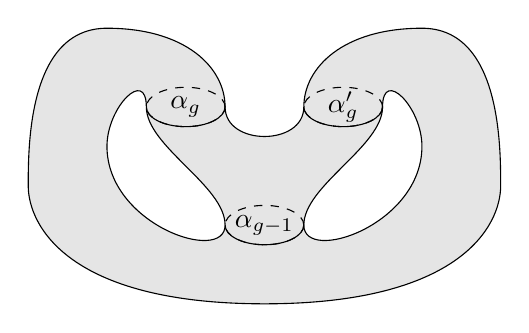
\begin{tikzpicture}





    \draw[fill=gray!20] (-0.5,1.5) .. controls (-1.5,1.5) and (-1.5,0) .. (-1.5,-0.5) .. controls (-1.5,-1) and (-1,-2) .. (1.5,-2) .. controls (4,-2) and  (4.5,-1) .. (4.5,-0.5) .. controls (4.5,0) and (4.5,1.5) .. (3.5,1.5) .. controls (2.5,1.5) and (2,1) .. (2,0.5) .. controls (2,0) and (1,0) .. (1,0.5) .. controls (1,1) and (0.5,1.5) .. (-0.5,1.5);
    \begin{scope}[]
    \draw[fill=white] (0,0.5) .. controls (0,1) and (-0.5,0.5) .. (-0.5,0) .. controls (-0.5,-1) and (1,-1.5) .. (1,-1) .. controls (1,-0.5) and (0,0) .. (0,0.5);
    
    \end{scope}
    \begin{scope}[xscale=-1, shift={(-3,0)}]
    \draw[fill=white] (0,0.5) .. controls (0,1) and (-0.5,0.5) .. (-0.5,0) .. controls (-0.5,-1) and (1,-1.5) .. (1,-1) .. controls (1,-0.5) and (0,0) .. (0,0.5);
    
    \end{scope}
    
    
    \begin{scope}[shift={(1,1.5)}]
    \draw[dashed]  (1.5,-1) ellipse (0.5 and 0.25);
    \clip  (2,-1) rectangle (1,-1.75);
    \draw  (1.5,-1) ellipse (0.5 and 0.25);
    \end{scope}
    
    
    \begin{scope}[shift={(0,0)}]
    \draw[dashed]  (1.5,-1) ellipse (0.5 and 0.25);
    \clip  (2,-1) rectangle (1,-1.75);
    \draw  (1.5,-1) ellipse (0.5 and 0.25);
    \end{scope}
    
    
    \begin{scope}[shift={(-1,1.5)}]
    \draw[dashed]  (1.5,-1) ellipse (0.5 and 0.25);
    \clip  (2,-1) rectangle (1,-1.75);
    \draw  (1.5,-1) ellipse (0.5 and 0.25);
    \end{scope}
    
    \node at (1.5,-1) {$\alpha_{g-1}$};
    \node at (0.5,0.5) {$\alpha_g$};
    \node at (2.5,0.5) {$\alpha_g'$};
    \end{tikzpicture}
%label:"thm:heegaardMoves"
%author:JeffHicks
%name:"Heegaard moves generate equivalences"
%type:"theorem"
%source:"singer1933three"


    \label{thm:heegaardMoves}
    Suppose that $(\Sigma_g,\underline \alpha, \underline \beta)$ and $(\Sigma_{g'},\underline \alpha', \underline \beta')$ are Heegaard diagrams for $M$. There exist a sequence of Heegaard moves and stabilizations taking one to the other. 

It follows that in order to construct 3-manifold invariants, one needs to find  quantities associated to the Heegaard diagram which are invariant under stabilizations, isotopies, and handles slides. Heegaard-Floer cohomology provides such an invariant.